%%%%%%%%%%%%%%%%%%%%%%%%%%%%%%%%%%%%%%%%%%%%%%%%%%%%%%%%%%%%
%%% ELIFE ARTICLE TEMPLATE
%%%%%%%%%%%%%%%%%%%%%%%%%%%%%%%%%%%%%%%%%%%%%%%%%%%%%%%%%%%%
%%% PREAMBLE 
\documentclass[9pt,lineno]{elife}
% Use the onehalfspacing option for 1.5 line spacing
% Use the doublespacing option for 2.0 line spacing
% Please note that these options may affect formatting.
% Additionally, the use of the \newcommand function should be limited.


\usepackage{lipsum} % Required to insert dummy text
\usepackage[version=4]{mhchem}
\usepackage{siunitx}
\DeclareSIUnit\Molar{M}

%%%%%%%%%%%%%%%%%%%%%%%%%%%%%%%%%%%%%%%%%%%%%%%%%%%%%%%%%%%%
%%% ARTICLE SETUP
%%%%%%%%%%%%%%%%%%%%%%%%%%%%%%%%%%%%%%%%%%%%%%%%%%%%%%%%%%%%
\title{Fast gradients for receptor-ligand RMSD}

\author[1*]{Evangelos Coutsias}
\author[2]{Peter K. Eastman}
\author[3]{John D. Chodera}

\affil[1]{Department of Applied Mathematics and Statistics, Stony Brook University, Stony Brook NY 11749}
\affil[2]{Department of Chemistry, Stanford University, Stanford, CA 94305}
\affil[3]{Computational and Systems Biology Program, Sloan Kettering Institute, Memorial Sloan Kettering Cancer Center, New York, NY 10065}

\corr{evangelos.coutsias@stonybrook.edu}{EC}

%%%%%%%%%%%%%%%%%%%%%%%%%%%%%%%%%%%%%%%%%%%%%%%%%%%%%%%%%%%%
%%% ARTICLE START
%%%%%%%%%%%%%%%%%%%%%%%%%%%%%%%%%%%%%%%%%%%%%%%%%%%%%%%%%%%%

\begin{document}

\maketitle

\begin{abstract}
Quaternions provide a straightforward and efficient way to evaluate the least-squares aligned RMSD and its gradient, but systems in which one subset of particles (such as a biomolecular receptor) is used for alignment and another subset (such as a ligand) is used to evaluate the RMSD present further challenges.
Here, we derive a simple and efficient approach to computing the gradient of the RMSD with respect to atomic positions for such a case, and describe an efficient GPU-enabled implementation in the open source software package OpenMM.
We illustrate the utility of this approach by using expanded ensemble umbrella sampling methods in ligand RMSD to compute the binding free energy of various guests to a supramolecular host.
\end{abstract}

%%%%%%%%%%%%%%%%%%%%%%%%%%%%%%%%%%%%%%%%%%%%%%%%%%%%%%%%%%%%%%%%%%%%%%%%%%%%%%%%%%%%%%%%%%%%%%%%%%%%%%
% INTRODUCTION
%%%%%%%%%%%%%%%%%%%%%%%%%%%%%%%%%%%%%%%%%%%%%%%%%%%%%%%%%%%%%%%%%%%%%%%%%%%%%%%%%%%%%%%%%%%%%%%%%%%%%%

\section{Introduction}

This work builds on the approach described in \cite{coutsias2004using}.

%%%%%%%%%%%%%%%%%%%%%%%%%%%%%%%%%%%%%%%%%%%%%%%%%%%%%%%%%%%%%%%%%%%%%%%%%%%%%%%%%%%%%%%%%%%%%%%%%%%%%%
% DERIVATION
%%%%%%%%%%%%%%%%%%%%%%%%%%%%%%%%%%%%%%%%%%%%%%%%%%%%%%%%%%%%%%%%%%%%%%%%%%%%%%%%%%%%%%%%%%%%%%%%%%%%%%

\section{Derivation}

This work builds on the notation used in \cite{coutsias2004using}.

Suppose we have a reference set of fe given an ordered set of vectors ${\bf y}_k$ 

After aligning a 
\begin{eqnarray}
N 
\end{eqnarray}


%%%%%%%%%%%%%%%%%%%%%%%%%%%%%%%%%%%%%%%%%%%%%%%%%%%%%%%%%%%%%%%%%%%%%%%%%%%%%
\section{Introduction}
%%%%%%%%%%%%%%%%%%%%%%%%%%%%%%%%%%%%%%%%%%%%%%%%%%%%%%%%%%%%%%%%%%%%%%%%%%%%%

We consider the problem of optimizing the RMSD of a substructure under optimal fit of two
structures and derive the relevant Jacobians.

Given template $\left[x,X\right]$ of protein+ligand and an ensemble of poses
$\left[y_i,Y_i\right]$ (perhaps a trajectory $\left[y(t),Y(t)\right]$, we drop the subscripts
in the sequel) how is shape+placement
of ligand affected by change in shape of protein? These have $n,N$ atoms, respectively 
involved in shape comparisons e.g. heavy atoms or some other given subset. 
Here we assume wlog that $x$ and $X$ viewed as sets of atom coordinate vectors are disjoint.
Throughout we write
$a_{jk}$ for the $j$-th component ($j=1,2,3$) of the $k$-th vector, ${\bf a}_k$.
We could use $3\times n$ matrices $x$ 
and $y$ where the $k$-th column of $x$ is the position vector 
${\bf x}_k$ of the k-th atom and similarly for $y$ (and also $3\times n$ matrices 
for $X, Y$ etc). 
To avoid tensor notation (as much as possible!) unfold these into $3n$ (resp. $3N$)
sized column vectors, and that is how we think of $x,X,y,Y$ below.

Some definitions:
\begin{enumerate}
\item $I_k$ is the $k\times k$ identity matrix.
\item ${\bf 1}_k$ is an $k\times 1$ array (column vector) of $1$'s.
\item ${\cal I}_{(k)} = {\bf 1}_n\otimes I_3$ is a $3k\times 3$ array with
$k$ blocks of $I_3$'s stacked as a block-column. 
\item $U(x,y)$ is the optimal rotation.
\item $\bar{\bf y} = \sfrac{1}{n} \sum_{k=1}^n {\bf y}_k $ is the centroid of $y$.
\item ${\cal I}_{(k)} {\bf a} := a_{(k)}$ is a $3k\times 1$ array of stacked
copies of vector $\bf a$.
\item ${\cal U}^{(k)} := I_k\otimes U$ is a k-block diagonal matrix of $U$'s.
\end{enumerate}

 The optimal superposition of $x$ with 
$y \rightarrow y' = {\cal U}^{(n)}*(y-\bar{y}_{(n)})$
(individual atom vectors are transformed as
${\bf y}_k^{\prime} = U*({\bf y}_k-\bar{\bf y})$;
the template is assumed to have centroid at 0),
minimizes the residual

\begin{equation}
\label{RMSD}
e(t) := RMSD^2\left(x,y\right) = \sfrac{1}{n}\left|x-y'\right|^2 = \sfrac{1}{n}\sum_{k=1}^n | {\bf x}_k -
 {\bf y}'_k |^2 \ .
\end{equation}

Based on the superposition (\ref{RMSD}), the ligand residual is
\be%\label{residual}
E(t) := \sfrac{1}{N}\left|X-Y'\right|^2 = 
\sfrac{1}{N}\left|X-{\cal U}^{(N)}(x,y)*(Y-{\bar y_{(N)}})\right|^2 \ .
\ee

We want to find $dE/dt$. That requires the Jacobian of $E$ with respect to $y$,
the coordinates of the realization (in the trajectory case, $dy/dt$ is known). 
There are two contributions:
\begin{eqnarray*}
(1) & \sfrac{\partial \bar{\bf y}}{\partial y} = 
\sfrac{1}{n} \sfrac{\partial \left(\sum_{k=1}^n {\bf y}_k\right)}{\partial y}  \\
(2) & \sfrac{\partial U}{\partial y} \ .
\end{eqnarray*}

%%%%%%%%%%%%%%%%%%%%%%%%%%%%%%%%%%%%%%%%%%%%%%%%%%%%%%%%%%%%%%%%%%%%%%%%%%%
\subsection{Derivative of mean position-in progress}
%%%%%%%%%%%%%%%%%%%%%%%%%%%%%%%%%%%%%%%%%%%%%%%%%%%%%%%%%%%%%%%%%%%%%%%%%%
\begin{eqnarray*}
\sfrac{\partial \bar{\bf y}}{\partial y}& = & 
\sfrac{1}{n} \sfrac{\partial \left(\sum_{k=1}^n {\bf y}_k\right)}{\partial y}  \\
\end{eqnarray*}
%%%%%%%%%%%%%%%%%%%%%%%%%%%%%%%%%%%%%%%%%%%%%%%%%%%%%%%%%%%%%%%%%%%%%%%%%%%
\subsection{Minimal residual background}
%%%%%%%%%%%%%%%%%%%%%%%%%%%%%%%%%%%%%%%%%%%%%%%%%%%%%%%%%%%%%%%%%%%%%%%%%%

We now promote ${\bf x}_k$ and ${\bf y}_k$ to {\em pure quaternions}
(see \ref{sec:quaternions}),
$x_k := (0, {\bf x}_k)$ with $x_k^c = - x_k$ and similarly for $y_k$.
The rotation ${\cal U}(q)$ on ${\bf y}_k$ is then written as
\[ \left( 0, {\cal U}(q) {\bf y}_k \right) = q y_k q^c. \] 
The residual is written, in terms of quaternions, as
\begin{equation}
E_q = \sfrac{1}{N}\sum_{k=1}^N \left( q y_k q^c - x_k\right)
\left(q y_k q^c - x_k\right)^c.
\label{resq}
\end{equation}
Expanding and multiplying by $N$, Eq.\ (\ref{resq}) becomes
\begin{eqnarray}
NE_q & = & \sum_{k=1}^N
\left( (q y_k q^c)(q y_k q^c)^c + x_k x_k^c - (q y_k q^c)x_k^c
-x_k (q y_k q^c)^c \right) \nonumber \\
& = & \sum_{k=1}^N\left(
x_k x_k^c + y_k y_k^c + (q y_k q^c)x_k + x_k (q y_k q^c) \right),
\label{qqq}
\end{eqnarray}
where use has been made of the normalization $q q^c = 1$ and the property
of pure quaternions $x^c = - x$. Since $q y_k q^c$ and $x_k$ are pure, and
for $a$, $b$ pure we have $ab + ba = 2(-{\bf a}\cdot{\bf b},{\bf 0})
= 2([ab]_0, {\bf 0}) $,
the last two terms in Eq.\ (\ref{qqq}) can be combined as:
\[ (q y_k q^c)x_k + x_k (q y_k q^c) =
2 (\left[ x_k (q y_k q^c) \right]_0, {\bf 0}),\]
i.e., only the 0th component is non-zero. We write
$x_k (q y_k q^c) = (x_k q y_k) q^c $ using the associativity of quaternions, 
and define $ z_k := x_k q y_k$. The 4-vector form of $z_k$, ${\cal Z}_k$,
can be written as ${\cal Z}_k = {\cal A}_L(x_k) {\cal A}_R(y_k) {\cal Q}$, where
${\cal A}_L(x_k)$ and ${\cal A}_R(y_k)$ are defined as in Eq.\ (\ref{eq38}).
Putting these together,
\bea
-2{\bf x}_k^T {\cal U}(q) {\bf y}_k & =  & 2\left[ x_k (q y_k q^c) \right]_0 
\nonumber\\
& = &  2 \left[ z_k q^c \right]_0 
 = 2 ({z_k}_0 q_0 + {\bf z}_k\cdot {\bf q})
\nonumber \\
& = & 2{\cal Q}^T {\cal Z}_k =
2{\cal Q}^T {\cal A}_L(x_k) {\cal A}_R(y_k) {\cal Q}. 
\label{4vec}
\eea

Collecting results, we find that the residual can be written as
\be
NE_q = \sum_{k=1}^N\left( |{\bf x}_k|^2 + |{\bf y}_k|^2 \right)
- 2{\cal Q}^T {\cal F} {\cal Q},
\ee
where
\[ {\cal F} := -\sum_{k=1}^N {\cal A}_L(x_k) {\cal A}_R(y_k). \]
The explicit form of the matrix ${\cal F}$ in terms of
the matrix elements of the moment matrix 
${\cal R}$ (\ref{eq:Kabsch}), 
\begin{equation}
\label{eq:Kabsch}
{\cal R} := {\cal Y}{\cal X}^T = \sum_{k=1}^N {\bf y}_k {\bf x}_k^T \rightarrow R_{ij} 
= \sum_{k=1}^N y_{ik} x_{jk} \ ,\ i,j=1,2,3
\ ,
\end{equation}
with $x_{ik}$ denoting the
$i$th component of ${\bf x}_k$, and likewise for $y_{jk}$.
is\\
${\cal F}=$
\begin{small}
\be
%{\cal F} = 
\left(
\begin{array}{cccc}
R_{11} + R_{22} + R_{33} & R_{23} - R_{32}
& R_{31} - R_{13} & R_{12} - R_{21} \\
R_{23} - R_{32} & R_{11} - R_{22} - R_{33}
& R_{12} + R_{21} & R_{13} + R_{31} \\
R_{31} - R_{13} & R_{12} + R_{21} 
& -R_{11} + R_{22} - R_{33} & R_{23} + R_{32} \\
R_{12} - R_{21} & R_{13} + R_{31} 
& R_{23} + R_{32} &-R_{11} - R_{22} + R_{33}
\end{array}
\right) \ .
\label{eq:F_explicit}
\ee
\end{small}

The problem has in this way been reduced to that of finding the extrema
of a quadratic form ${\cal Q}^T {\cal F} {\cal Q}$ in the four variables 
$q_i$, $i = 0,1,2,3$, subject to the constraint ${\cal Q}^T {\cal Q} =1$. 
Note that here we are using the vector ${\cal Q}$, so that the squared norm
$q^cq$ is written equivalently as ${\cal Q}^T{\cal Q}$. 
${\cal Q}^T {\cal F} {\cal Q}$ is the standard Rayleigh quotient 
for a symmetric matrix ${\cal F}$, 
and the maximum value achieved by ${\cal Q}^T {\cal F} {\cal Q}$ is 
equal to its largest eigenvalue. 
Thus, the desired minimization leads to the eigenproblem
\be
{\cal F} {\cal Q} = \lambda {\cal Q}.
\label{eig}
\ee
We see that the extremum $\lambda$ is equal to one of the 
eigenvalues of a
$4\times 4$ symmetric, traceless matrix, and the corresponding eigenvector
gives one of the candidate rotations that extremize the residual, as
sought. 
We are thus led to the following expression for the best-fit RMSD $e_q$:
\[ 
e_q = \sqrt{\min_{||q||=1} E_q} = 
\sqrt{
\sfrac{\sum_{k=1}^N
\left( |{\bf x}_k|^2 + |{\bf y}_k|^2 \right) - 
2 \lambda_{\mbox{\scriptsize{max}}}}{N}},
\] 
where $\lambda_{\mbox{\scriptsize{max}}}$ is the maximum eigenvalue of
$\cal F$. If a rotation reflection is allowed, then the minimal eigenvalue
$\lambda_4$ must also be considered. If $-\lambda_4 > \lambda_1$, then
the improper rotation $-{\cal U}(q_4)$ will give a better fit than the
proper rotation ${\cal U}(q_1)$ (see \ref{sec:quaternions}, 
eq.(\ref{eq35}) for the
construction of the rotation matrix ${\cal U}(q)$ from the quaternion $q$). 
This is easily seen, since the matrix
${\cal F}$ is linear in both ${\cal X}$ and ${\cal Y}$, therefore
the substitution ${\cal X} \rightarrow -{\cal X}$ changes the sign of the
eigenvalues. 
%
%%%%%%%%%%%%%%%%%%%%%%%%%%%%%%%%%%%%%%%%%%%%%%%%%%%%%%%%%%%%%%%%%%%%%%%%%%%%%%
\section{Gradient of the RMSD and optimal rotation matrix}
%\section{Gradient of the RMSD and application to an optimization problem}
\label{sec:grad}
%%%%%%%%%%%%%%%%%%%%%%%%%%%%%%%%%%%%%%%%%%%%%%%%%%%%%%%%%%%%%%%%%%%%%%%%%%%%%
{\bf NOTE: needs lots of work}

The gradient of the RMSD with respect to the model coordinates is required
in several applications. For simplicity here we work with $E= e ^2$. 
It is well known \cite{brooks1} that the gradient
is equal to the residual vector in the form,
\begin{equation}
\label{eq:grad-charmm}
 \nabla_y {e} = \sfrac{2}{N}\sum_{k=1}^N {\bf x}_k - U {\bf y}_k \ 
\end{equation}
Previously \cite{Coutsias2003} we gave
a simple derivation using the quaternion formalism,
and presented a calculation
using the gradient to find the best-fit reduced model
to a target structure.

We consider the case in which the model coordinates ${\bf x}_k$ are functions of
a parameter set ${\alpha}$. The parameter set $\alpha$ could be an energy 
parameter set that places
${\bf x}_k(\alpha)$ at the global energy minimum, or a set of geometrical
variables that represents a reduced structure model.
By the chain rule,
\[ 
\sfrac{\partial e}{\partial \alpha_i} = 
\sum_{k=1}^{N}\sum_{l=1}^{3}\sfrac{\partial E}{\partial x_{lk}}
\sfrac{\partial x_{lk}}{\partial \alpha_i},
\]
where $x_{lk}$ is the $l$th component of ${\bf x}_k$, and $\alpha_i$ is the
$i$th component of $\alpha$.
For the second factor ${\partial E}/{\partial x_{lk}}$ we use the results
derived in the previous section. Since 
\begin{equation}
\label{grad}
 \sfrac{\partial E}{\partial x_{lk}} = \sfrac{2}{N}
\left(x_{lk} - \sfrac{\partial 
\lambda_{\mbox{\scriptsize{max}}}}{\partial x_{lk}} \right), 
\end{equation}
we need formulas for the quantities ${\partial \lambda_{\mbox{\scriptsize{j}}}}/{\partial x_{lk}}$. 

We review a simple calculation from matrix perturbation theory
\cite{StSu}:\\
{\bf Problem:}
{\em Let $M(t)$ be a symmetric matrix, whose coefficients depend
differentiably on the
parameter $t$. Find expressions for the variation of its eigenvalues
and eigenvectors with respect to $t$, i.e., $(\lambda_t, {\bf v}_t)$. }\\
{\bf Solution: }
We write
\[ M V = V \Lambda, \]
where
\[ \Lambda = diag(\lambda_1, \lambda_2, \ldots,\lambda_N), \]
and we assume $\lambda_i \ne \lambda_j$ for $i \ne j$.
The eigenvectors are orthonormal, $V V^T = I$. Since the columns of $V$
form a complete, orthonormal set, we can write:
\be
\sfrac{d V}{d t} = V A,
\label{eq:a}
\ee
for some matrix $A$,
i.e., the $d{\bf v}_i/dt$ are written as linear combinations of the
${\bf v}_i$'s. Since $V^T V = I$ we have
\[ \sfrac{d V^T}{d t} V + V^T \sfrac{d V}{d t} = 0 \rightarrow A^T + A = 0, \]
so that the matrix $A$ is skew, $A^T = -A$, which is to be expected since
$A$ is the generator of a rotation.
Then, from $M = V \Lambda V^T $ we have
\begin{eqnarray*}
\sfrac{d M}{d t} & = & \sfrac{d V}{d t}\Lambda V^T +
V \sfrac{d\Lambda}{d t} V^T +
V \Lambda \sfrac{d V^T}{d t} \\
& = & V \left\{ \sfrac{d\Lambda}{d t} + A\Lambda + \Lambda A^T
\right\} V^T,
\end{eqnarray*}
so that, finally:
\be
\label{evol}
V^T \sfrac{d M}{d t} V = \sfrac{d\Lambda}{d t} + A\Lambda - \Lambda A.
\ee


From the general results given above,
\[ V^T \sfrac{\partial {\cal F}}{\partial x_{lk}} V =
\sfrac{\partial \Lambda}{\partial x_{lk}} + A\Lambda - \Lambda A, \]
where the eigenvalue matrix $\Lambda$, the eigenvector matrix $V$, and
the generator matrix of rotation $A$ are defined in Appendix A.
Since the diagonal elements of $A\Lambda - \Lambda A$ vanish we have
\begin{equation}
\label{eq:grad-eval}
 \sfrac{\partial \lambda_{\mbox{\scriptsize{j}}}}{\partial x_{lk}} =
{\cal Q}^T_j \sfrac{\partial {\cal F}}{\partial x_{lk}} 
{\cal Q}_j\ , 
\end{equation} 
where ${\cal Q}_j\equiv {\cal Q}_{\mbox{\scriptsize{j}}}$ is the normalized 
eigenvector corresponding 
to the eigenvalue $\lambda_{\mbox{\scriptsize{j}}}$.
%To show that this formula leads to eq.(\ref{eq:grad-charmm}) we recall that
%$q^c y_k q = (0, {\cal U}^T(q){\bf y}_k)$.
% and use the identity
%$ \left(ab\right)_0 = \left(ba\right)_0 $. 
%Writing as above $q\equiv q_{\mbox{\scriptsize{j}}}$ for the quaternion 
%equivalent
%to the eigenvector ${\cal Q}_{\mbox{\scriptsize{j}}}$, and fixing its value in
%dealing with the gradient operator as a matter of algebraic convenience
%we have, using eq.(\ref{4vec}): 
%\begin{eqnarray}
% \nabla_{{\bf x}_k} \lambda_{\mbox{\scriptsize{max}}}
%& = & {\cal Q}^T \nabla_{{\bf x}_k} {\cal F} 
%{\cal Q} = \nabla_{{\bf x}_k} 
%\left(-{\cal Q}^T {\cal A}_L(y_k){\cal A}_R(x_k)
%{\cal Q}\right) \nonumber \\
% & = & 
%\nabla_{{\bf x}_k}\left( {\bf y}_k^T {\cal U}(q) 
%{\bf x}_k \right) 
% = \nabla_{{\bf x}_k} \left(  {\bf x}_k^T {\cal U}^T {\bf y}_k \right)
%= {\cal U}^T {\bf y}_k 
%\label{result}
%\end{eqnarray}
%so that (\ref{grad}) is equivalent to (\ref{eq:grad-charmm}).
% and
%\[ 
%\frac{\partial {\cal F}}{\partial x_{1k}} =
%\left(
%\begin{array}{rrrr}
% y_{1k} &  0     & -y_{3k} &  y_{2k} \\
%      0 & y_{1k} &  y_{2k} &  y_{3k} \\
%-y_{3k} & y_{2k} & -y_{1k} &      0  \\
% y_{2k} & y_{3k} &       0 & -y_{1k} 
%\end{array}
%\right), 
%\]
%\[ \frac{\partial {\cal F}}{\partial x_{2k}} =
%\left(
%\begin{array}{rrrr}
% y_{2k} &  y_{3k} &      0 & -y_{1k} \\
% y_{3k} & -y_{2k} & y_{1k} &       0 \\
%      0 &  y_{1k} & y_{2k} &  y_{3k} \\
%-y_{1k} &       0 & y_{3k} & -y_{2k} 
%\end{array}
%\right), 
%\]
%\be
%\frac{\partial {\cal F}}{\partial x_{3k}} =
%\left(
%\begin{array}{rrrr}
% y_{3k} & -y_{2k} &  y_{1k} &      0 \\
%-y_{2k} & -y_{3k} &       0 &  y_{1k} \\
% y_{1k} &       0 & -y_{3k} &  y_{2k} \\
%      0 &  y_{1k} &  y_{2k} &  y_{3k} 
%\end{array}
%\right). 
%\label{eq:dF_dx}
%\ee 
These formulas hold assuming the eigenvalues are distinct (degeneracy requires
special treatment, not given here). Under the same assumption, 
we seek now expressions for the variation of the eigenvectors, which 
necessitates looking at the off-diagonal elements of eq.(\ref{evol}).

Now
\[ A \Lambda - \Lambda A =
\left(
\begin{array}{cccc}
0 & (\lambda_2-\lambda_1)a_{12} & (\lambda_3-\lambda_1)a_{13}&(\lambda_4-\lambda_1)a_{14}\\
(\lambda_2-\lambda_1)a_{12} &0&(\lambda_3-\lambda_2)a_{23}&(\lambda_4-\lambda_2)a_{24}\\
(\lambda_3-\lambda_1)a_{13}&(\lambda_3-\lambda_2)a_{23}&0&(\lambda_4-\lambda_3)a_{34}\\
(\lambda_4-\lambda_1)a_{14}&(\lambda_4-\lambda_2)a_{24}&(\lambda_4-\lambda_3)a_{34}& 0
\end{array} \right)
\]
so that
\begin{eqnarray*}
a_{ii} & = & 0 \\
a_{ij} & = & \sfrac{1}{\lambda_j - \lambda_i}q_i^T\sfrac{d{\cal F}}{dt}q_j
\end{eqnarray*}

which is what we needed for computing $dU/dt$: using the formulas in the Appendix,
\[ \left(
\begin{array}{cc}
1 & {\bf 0}^T \\
{\bf 0} & {\cal U}(q_1) 
\end{array}
\right)
= {\cal A}_L(q_1) {\cal A}_R(q_1^c). \]
with
\[\sfrac{dq_1}{dt} = V\left(
\begin{array}{c}
0 \\
(\lambda_2-\lambda_1)a_{12} \\
(\lambda_3-\lambda_1)a_{13}\\
(\lambda_4-\lambda_1)a_{14}
\end{array} \right)
\]
({\bf to be continued}).
%Near a degeneracy in the leading eigenvalue (i.e. if $\lambda_1 \approx
%\lambda_2 > 0$), the one parameter family of rotations
%\[ {\cal U}(q(t)) := {\cal U}\left(\cos{t} q_1 + \sin{t} q_2 
%\right)\ ,\ 0\le t <2\pi \]
%produces near minimal residual for all values of the parameter $t$.
%Of course, at the point of degeneracy, all
%such rotations produce equal, and minimal, residuals since $q(t)$ is also
%a unit eigenvector of eigenvalue $\lambda_{\mbox{\scriptsize{max}}}$.
%In this case, the precise choice of optimal superposition needs to be
%made keeping in mind any additional requirements inherent in a given
%situation. For example, in the Nudged Elastic Band method \cite{brooks1}
%the above form could serve as an optimal switching function between
%branches near a degeneracy that would avoid large force fluctuations while
%remaining close to optimal superposition at all times.

%%%%%%%%%%%%%%%%%%%%%%%%%%%%%%%%%%%%%%%%%%%%%%%%%%%%%%%%%%%%%%%%%%%%%%%%%%%%%
\appendix
\def\thesection{Appendix \Alph{section}} 
%%%%%%%%%%%%%%%%%%%%%%%%%%%%%%%%%%%%%%%%%%%%%%%%%%%%%%%%%%%%%%%%%%%%%%%%%%%%%
%%%%%%%%%%%%%%%%%%%%%%%%%%%%%%%%%%%%%%%%%%%%%%%%%%%%%%%%%%%%%%%%%%%%%%%%%%%%%
\section{Quaternion notation and properties}
\label{sec:quaternions}
%%%%%%%%%%%%%%%%%%%%%%%%%%%%%%%%%%%%%%%%%%%%%%%%%%%%%%%%%%%%%%%%%%%%%%%%%%%%%

We review basic properties of quaternions below. We follow the notes 
of Coutsias and Romero \cite{notes}, and refer the reader to these notes 
for more
details. The book by Rappaport \cite{rap}, which discusses quaternions in the 
context of molecular dynamics, is also useful as an introduction.
We define a quaternion $q$ as a 4-vector $q=(q_0,q_1,q_2,q_3)
\equiv(q_0,{\bf q})$, where ${\bf q} = (q_1,q_2,q_3)$, 
with the obvious addition law and the fundamental multiplication law given by
\bea
a = (a_0, {\bf a}), &\quad& b = (b_0, {\bf b}), \nonumber \\
a+b &=& (a_0+b_0, {\bf a}+{\bf b}), \nonumber \\
\label{eq26}
a\,b &=& (a_0 b_0 - {\bf a}\cdot{\bf b},
a_0 {\bf b}+b_0 {\bf a}+ {\bf a}\times{\bf b}), 
\eea 
where the multiplication can be seen to be associative, $a(bc) = (ab)c$,
but not commutative, $ab \ne ba$, in general.
We also define the \textit{conjugate} quaternion $q^c$, the squared norm of a 
quaternion $N(q)$, and the inverse quaternion $q^{-1}$ by
\bea
\label{eq27}
q^c &:=& (q_0,-{\bf q}), \qquad (a b)^c = b^c a^c, \\
\label{eq28}
N(q) &:=& q^cq = qq^c = q_0^2+{\bf q}\cdot{\bf q}, \\
\label{eq29}
q^{-1} &:=& \frac{q^c}{N(q)} = \frac{(q_0,-{\bf q})}{N(q)}. 
\eea 

An important class of quaternions is the \textit{pure} quaternions 
which have the form $q = (0,{\bf q})$.
Pure quaternions can be considered as ordinary 3-vectors 
${\bf q}=(q_1,q_2,q_3)$ which have been mapped to 4-vectors,
$(0,{\bf q}) = (0,q_1,q_2,q_3)$. 
Note for pure quaternions $a,b$, \eq{26} and \eq{27} yield
\bea
\label{eq31}
a = (0,\bbox{a}), &\quad& b = (0,\bbox{b}), \nonumber \\
a\,b &=& (-\bbox{a}\cdot\bbox{b}, \, \bbox{a}\times\bbox{b}), \\
\label{eq32}
a^c &=& (0,-\bbox{a}) = -a.
\eea 

The quaternion product can be formulated
as a matrix multiplication as follows:
\bea
\label{eq36}
pq & =: & {\cal A}_L(p) {\cal Q}, \qquad \textrm{ $p$ operates 
on $q$ from the left,}\\
\label{eq37}
qp & =: & {\cal A}_R(p) {\cal Q}, \qquad \textrm{ $p$ operates on 
$q$ from the right,}
\eea
where ${\cal A}_L(p)$ and ${\cal A}_R(p)$ are $4\times 4$ matrices, 
and ${\cal Q}=(q_0,q_1,q_2,q_3)^T$ is the column 4-vector representation
of quaternion $q$.
By convention, the matrix multiplication form of the quaternion product 
(the right-hand side of the above) 
is defined to act from the left on a column 4-vector.
For $p=(p_0,p_1,p_2,p_3)$ the matrices ${\cal A}_L(p)$ and 
${\cal A}_R(p)$ are given by
\be
{\cal A}_R(p) = \left( 
\begin{array}{cccc}
p_0 & -p_1 & -p_2 & -p_3 \\
p_1 & p_0 & p_3 & -p_2 \\
p_2 & -p_3 & p_0 & p_1 \\
p_3 & p_2 & -p_1 & p_0
\end{array}
\right),
\quad
{\cal A}_L(p) = \left( 
\begin{array}{cccc}
p_0 & -p_1 & -p_2 & -p_3 \\
p_1 & p_0 & -p_3 & p_2 \\
p_2 & p_3 & p_0 & -p_1 \\
p_3 & -p_2 & p_1 & p_0
\end{array}
\right).
\label{eq38}
\ee 

Quaternions provide a natural coordinate system for ${\cal SU}(3)$, the 
group of proper rotations of 3-space. Thus they can describe rotations without 
the singularities of, say, the Euler angles rotation matrices. For the 
3-vector $\bbox{r}'$ obtained by a rotation of the vector $\bbox{r}$ 
via the orthogonal rotation matrix ${\cal{U}}$ we have
\bea
\label{eq33}
r' = (0,{\bf r}'), &\quad& r = (0,{\bf r}), \nonumber \\
r' &=& q \, r \, q^c, \\
\label{eq34}
(0,\bbox{r'}) &=& (q_0,{\bf q}) \; (0,\bbox{r}) \; (q_0, -{\bf q}) 
\nonumber \\ &=& (0,\, {{\cal{U}}(q)}\bbox{r}).
\eea 
Using the notation of Eq.\ (\ref{eq38}), we can express the rotation matrix 
as a product of two matrices, each depending linearly on a unit quaternion $q$
($qq^c = 1$):
\[ \left(
\begin{array}{cc}
1 & {\bf 0}^T \\
{\bf 0} & {\cal U}(q) 
\end{array}
\right)
= {\cal A}_L(q) {\cal A}_R(q^c). \]
%(One must keep in mind when mixing matrices and quaternions that
%\textit{quaternion operations are not associative with 
%ordinary $4\times 4$ matrix multiplications}). 
The $3 \times 3$ rotation matrix ${\cal{U}}$ is given by
\be
{\cal{U}}(q) = 
\left(
\begin{array}{ccc}
q_0^2 + q_1^2-q_2^2-q_3^2 & 2(q_1 q_2-q_0 q_3)      & 2(q_1 q_3+q_0 q_2) \\
2(q_1 q_2+q_0 q_3)        & q_0^2-q_1^2+q_2^2-q_3^2 & 2(q_2 q_3-q_0 q_1) \\
2(q_1 q_3-q_0 q_2)        & 2(q_2 q_3+q_0 q_1)      & q_0^2-q_1^2-q_2^2+q_3^2
\end{array}
\right)\ .
\label{eq35}
\ee
Since ${\cal{U}}$ is orthogonal we have ${\cal{U}}^{-1} = {\cal{U}}^T$.
Note that by its construction, ${\cal{U}}(q)$ is a proper rotation whose
angle $\theta$ and axis ${\bf c}$ are seen in the form of $q$ 
\cite{notes, rap}:
\[ q = (q_0, {\bf q}) = (\cos{(\theta/2)}, \sin{(\theta/2)} {\bf c}). \]
It is easy to see that $\left\{ \theta, {\bf c} \right\}$ and 
$\left\{ -\theta, -{\bf c} \right\}$
produce the same quaternion $q$ and hence the same rotation. 
Also, $q$ and $-q$ produce the same rotation, a fact easily deduced from
the form of the rotation matrix ${\cal{U}}(q)$. 

%%%%%%%%%%%%%%%%%%%%%%%%%%%%%%%%%%%%%%%%%%%%%%%%%%%%%%%%%%%%%%%%%%%%%%%%%%%%%%%%%%%%%%%%%%%%%%%%%%%%%%
% Code and Data Availability
%%%%%%%%%%%%%%%%%%%%%%%%%%%%%%%%%%%%%%%%%%%%%%%%%%%%%%%%%%%%%%%%%%%%%%%%%%%%%%%%%%%%%%%%%%%%%%%%%%%%%%

\section{Code and data availability}

\begin{itemize}
\item Numpy examples
\item Code for this project is implemented in OpenMM \href{https://github.com/pandegroup/openmm}{https://github.com/pandegroup/openmm}. Documentation and installation instructions are available at \url{http://openmm.org}
\end{itemize}

%%%%%%%%%%%%%%%%%%%%%%%%%%%%%%%%%%%%%%%%%%%%%%%%%%%%%%%%%%%%%%%%%%%%%%%%%%%%%%%%%%%%%%%%%%%%%%%%%%%%%%
% Author Contributions 
%%%%%%%%%%%%%%%%%%%%%%%%%%%%%%%%%%%%%%%%%%%%%%%%%%%%%%%%%%%%%%%%%%%%%%%%%%%%%%%%%%%%%%%%%%%%%%%%%%%%%%
\section{Author Contributions}

Conceptualization, EC, JDC; 
Methodology, EC, PKE; 
Software, PKE; 
Formal Analysis, EC; 
Investigation, EC, JDC; 
Resources, EC, PKE, JDC;  
Data Curation, JDC; 
Writing-Original Draft, JDC; 
Writing - Review and Editing, EC, PKE, JDC; 
Visualization, JDC; 
Supervision, EC, PKE, JDC; 
Project Administration, EC, JDC; 
Funding Acquisition, EC, JDC

(Follow the \href{http://www.cell.com/pb/assets/raw/shared/guidelines/CRediT-taxonomy.pdf}{CRediT Taxonomy})

%%%%%%%%%%%%%%%%%%%%%%%%%%%%%%%%%%%%%%%%%%%%%%%%%%%%%%%%%%%%%%%%%%%%%%%%%%%%%%%%%%%%%%%%%%%%%%%%%%%%%%
% Acknowledgments 
%%%%%%%%%%%%%%%%%%%%%%%%%%%%%%%%%%%%%%%%%%%%%%%%%%%%%%%%%%%%%%%%%%%%%%%%%%%%%%%%%%%%%%%%%%%%%%%%%%%%%%
\section{Acknowledgments}

%JDC acknowledges support from NIH grant P30 CA008748 and the Sloan Kettering Institute.

%%%%%%%%%%%%%%%%%%%%%%%%%%%%%%%%%%%%%%%%%%%%%%%%%%%%%%%%%%%%%%%%%%%%%%%%%%%%%%%%%%%%%%%%%%%%%%%%%%%%%%
% Disclosures 
%%%%%%%%%%%%%%%%%%%%%%%%%%%%%%%%%%%%%%%%%%%%%%%%%%%%%%%%%%%%%%%%%%%%%%%%%%%%%%%%%%%%%%%%%%%%%%%%%%%%%%
\section{Disclosures}


%%%%%%%%%%%%%%%%%%%%%%%%%%%%%%%%%%%%%%%%%%%%%%%%%%%%%%%%%%%%%%%%%%%%%%%%%%%%%%%%%%%%%%%%%%%%%%%%%%%%%%
%%% BIBLIOGRAPHY
%%%%%%%%%%%%%%%%%%%%%%%%%%%%%%%%%%%%%%%%%%%%%%%%%%%%%%%%%%%%%%%%%%%%%%%%%%%%%%%%%%%%%%%%%%%%%%%%%%%%%%

%\nocite{*} % This command displays all refs in the bib file. PLEASE DELETE IT BEFORE YOU SUBMIT YOUR MANUSCRIPT!
%\bibliography{manual}

%%%%%%%%%%%%%%%%%%%%%%%%%%%%%%%%%%%%%%%%%%%%%%%%%%%%%%%%%%%%%%%%%%%%%%%%%%%%%
% REFERENCES 
%%%%%%%%%%%%%%%%%%%%%%%%%%%%%%%%%%%%%%%%%%%%%%%%%%%%%%%%%%%%%%%%%%%%%%%%%%%%%

\begin{thebibliography}{99} 
\bibitem{brooks1} Chu, J- W.; Trout, B.\ L.; Brooks, B.\ R. J.\
Chem.\ Phys.\ 2003, 119, 12708.
\bibitem{Coutsias2003} Coutsias, E.\ A.; Seok, C.;Dill, K.\ A.
sJ Comput Chem 25: 1849–1857, 2004.
\bibitem{StSu} Stewart, G.\ W.; Sun, J.-G. Matrix Perturbation
Theory; Academic Press: New York, 1990.
\bibitem{notes} Coutsias, E.\ A.; Romero, L.
The Quaternions with applications to Rigid Body Dynamics,
Sandia National Laboratories, 2004,
Technical Report SAND2004-0153.
\bibitem{rap} Rappaport, D.\ C. The Art of Molecular Dynamics 
Simulation; Cambridge Univ.\ Press: New York, 1995, Chapter 8, pp. 191-221.
\end{thebibliography} 


%%%%%%%%%%%%%%%%%%%%%%%%%%%%%%%%%%%%%%%%%%%%%%%%%%%%%%%%%%%%
%%% APPENDICES
%%%%%%%%%%%%%%%%%%%%%%%%%%%%%%%%%%%%%%%%%%%%%%%%%%%%%%%%%%%%

% \appendix
% \begin{appendixbox}
% \label{first:app}
% \section{Firstly}
% \lipsum[1]

% %% Sadly, we can't use floats in the appendix boxes. So they don't "float", but use \captionof{figure}{...} and \captionof{table}{...} to get them properly caption.
% \begin{center}
% 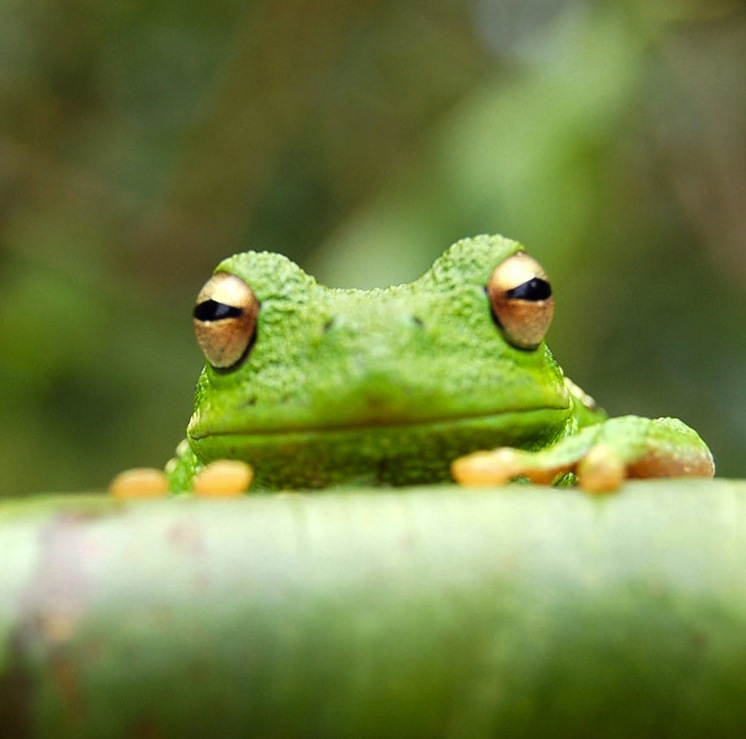
\includegraphics[width=\linewidth,height=7cm]{frog}
% \captionof{figure}{This is a figure in the appendix}
% \end{center}

% \section{Secondly}

% \lipsum[5-8]

% \begin{center}
% 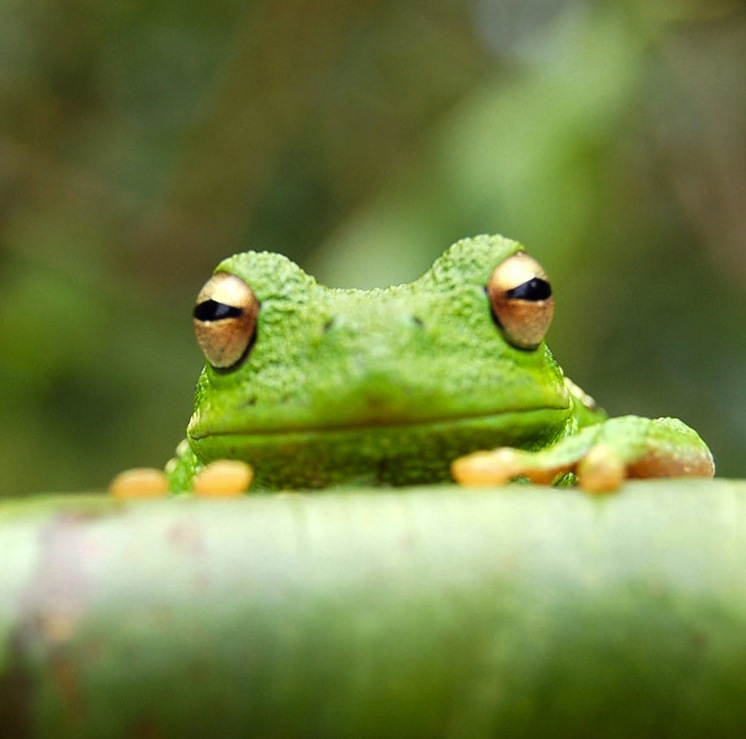
\includegraphics[width=\linewidth,height=7cm]{frog}
% \captionof{figure}{This is a figure in the appendix}
% \end{center}

% \end{appendixbox}

% \begin{appendixbox}
% 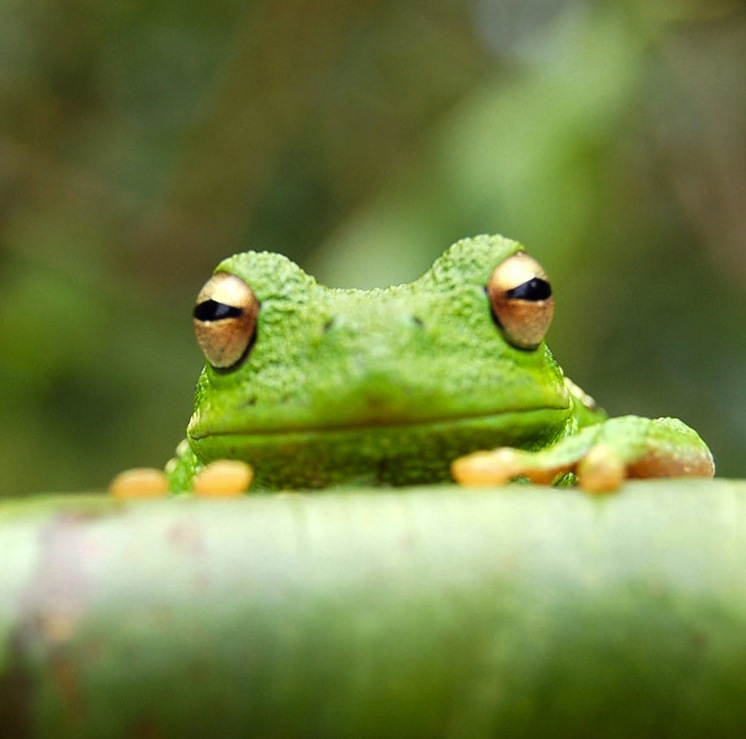
\includegraphics[width=\linewidth,height=7cm]{frog}
% \captionof{figure}{This is a figure in the appendix}
% \end{appendixbox}


\end{document}
